\documentclass{beamer}
\usepackage{graphicx}
\usepackage{epstopdf}
\usepackage{hyperref}
\usepackage{tikz}
\usepackage{listings}
\usepackage{subfig}

\usetikzlibrary{
    chains,
    positioning,
    arrows.meta,
    decorations.pathreplacing,
    calc,
    fit,
    shapes.geometric
}
                    
\graphicspath{ {images/} }

\bibliographystyle{plain}

\usetheme{Boadilla}

% https://latex.org/forum/viewtopic.php?t=6662
\setbeamertemplate{footline}
{
   \leavevmode%
   \hbox{%
   \begin{beamercolorbox}[wd=.333333\paperwidth,ht=2.25ex,dp=1ex,center]{author in head/foot}%
     \usebeamerfont{author in head/foot}\insertshortauthor%~~(\insertshortinstitute)
   \end{beamercolorbox}%
   \begin{beamercolorbox}[wd=.333333\paperwidth,ht=2.25ex,dp=1ex,center]{title in head/foot}%
     \usebeamerfont{title in head/foot}\insertshorttitle
   \end{beamercolorbox}%
   \begin{beamercolorbox}[wd=.333333\paperwidth,ht=2.25ex,dp=1ex,right]{date in head/foot}%
     \usebeamerfont{date in head/foot}\insertshortdate{}\hspace*{2em}
     \insertframenumber{} / \inserttotalframenumber\hspace*{2ex}
   \end{beamercolorbox}}%
   \vskip0pt%
}

\title{CS4099 Demo}
\subtitle{Ubiquitous Communication for the Internet of Things\\An Identifier-Locator addressing split overlay network}
\author{Ryan Gibb}
\institute{School of Computer Science\\University of St Andrews}
\titlegraphic{
\includegraphics[scale=2,trim={0.45cm 0.75cm 0.45cm 0.45cm},clip]{st_a_logo.eps}}

\date{Monday 19th April}

\AtBeginSection[]{
  \begin{frame}
  \vfill
  \centering
  \begin{beamercolorbox}[sep=8pt,center,shadow=true,rounded=true]{title}
    \usebeamerfont{title}\insertsectionhead\par%
  \end{beamercolorbox}
  \vfill
  \end{frame}
}

\begin{document}

\begin{frame}
	\maketitle
\end{frame}

\section{Section}


\begin{frame}{Background}[allowframebreaks]
\begin{itemize}
    \item Ubiquitous Computing and the Internet of Things (IoT)
    \pause
    \item Mobility in IP
    \begin{itemize}
        \item Overloading of IP address semantics
        \item Entanglement of layers
    \end{itemize}
    \pause
    \item Identifier-Locator Network Protocol (ILNP)
    \pause
\end{itemize}
\end{frame}




\begin{frame}{Discovery Protocol Example}
\begin{figure}[ht]
    \centering
    \makebox[\textwidth]{
        \begin{tabular}{c}            
            \subfloat[Network Topology \label{fig:discovery_topology}]
                {\scalebox{0.4}{
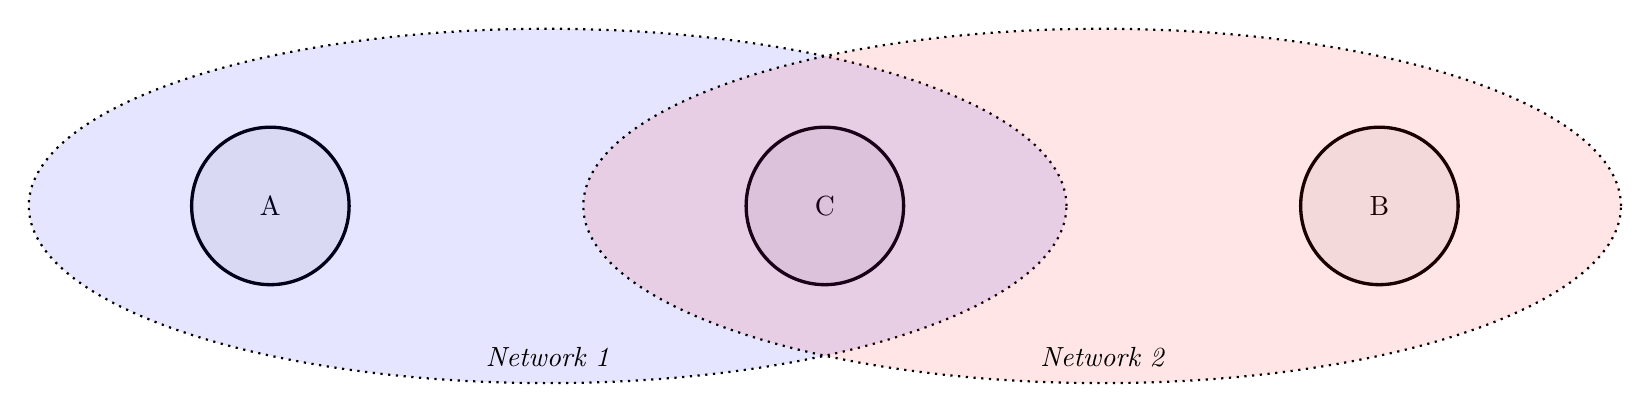
\begin{tikzpicture}[
    nwknode/.style={
        circle,
        very thick,
        minimum size=2cm,
        draw,
        fill=black!5,
    },
    network/.style args = {#1/#2}{
        ellipse,
        minimum height=4.5cm,
        draw,
        thick,
        dotted,
        fill=#1,
        fill opacity=0.1,
        text opacity=1,
        label={[anchor=south,above=1mm]270:{\itshape Network #2}}
    },
]
    \node[nwknode] (A) {A};
    \node[nwknode] (C) [right=5cm of A] {C};
    \node[nwknode] (B) [right=5cm of C] {B};
    
    \node[network={blue/1}, fit=(A)(C)] (net1) {};
    \node[network={red/2},  fit=(C)(B)] (net2) {};

\end{tikzpicture}}} \\
            \subfloat[Sequence Diagram \label{fig:discovery_sequence}]
                {\scalebox{0.4}{
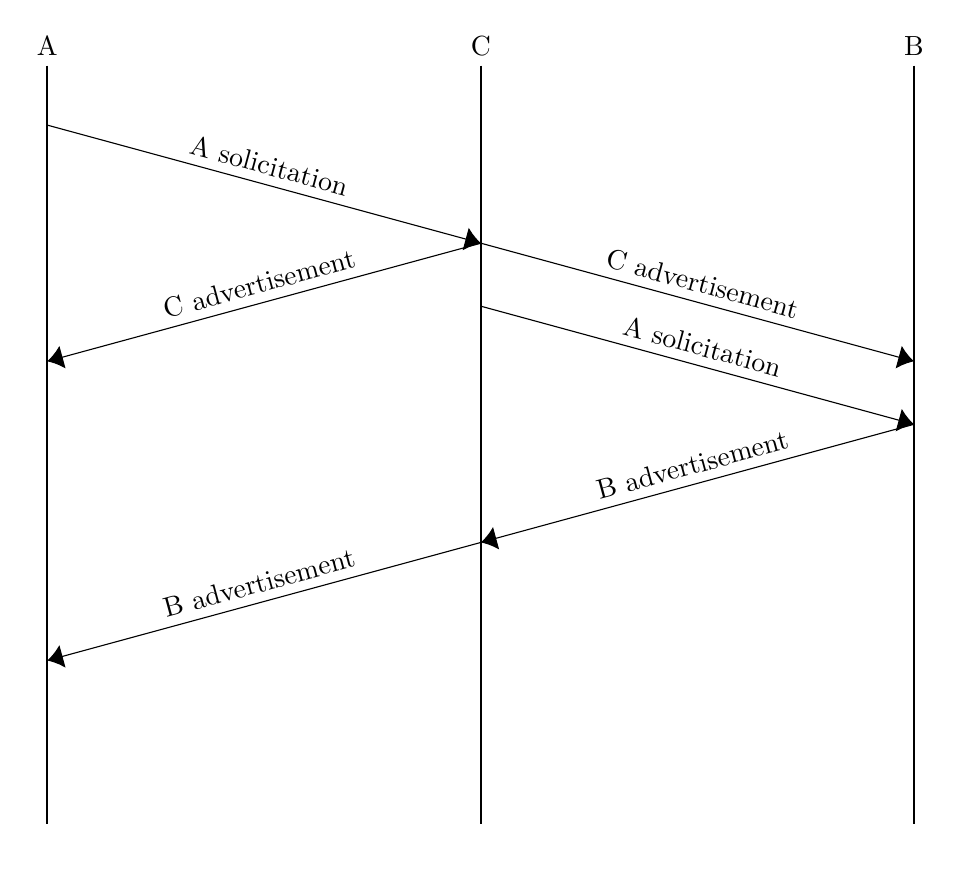
\begin{tikzpicture}[node distance=5cm,auto]
    \node[] (c) {C};
    \node[right = of c] (b) {B};
    \node[left = of c] (a) {A};
    \node[below of=c, node distance=10cm] (c_ground) {};
    \node[below of=b, node distance=10cm] (b_ground) {};
    \node[below of=a, node distance=10cm] (a_ground) {};
    
    \draw[thick] (c) -- (c_ground);
    \draw[thick] (b) -- (b_ground);
    \draw[thick] (a) -- (a_ground);
    
    \draw[-{Latex[length=2mm,width=3mm]}] ($(a)!0.1!(a_ground)$) -- node[above,sloped]{A solicitation}  ($(c)!0.25!(c_ground)$);
    
    \draw[-{Latex[length=2mm,width=3mm]}] ($(c)!0.25!(c_ground)$) -- node[above,sloped]{C advertisement} ($(b)!0.4!(b_ground)$);
    \draw[-{Latex[length=2mm,width=3mm]}] ($(c)!0.25!(c_ground)$) -- node[above,sloped]{C advertisement} ($(a)!0.4!(a_ground)$);
    
    \draw[-{Latex[length=2mm,width=3mm]}] ($(c)!0.33!(c_ground)$) -- node[above,sloped]{A solicitation} ($(b)!0.48!(b_ground)$);
    
    \draw[-{Latex[length=2mm,width=3mm]}] ($(b)!0.48!(b_ground)$) -- node[above,sloped]{B advertisement} ($(c)!0.63!(c_ground)$);
    \draw[-{Latex[length=2mm,width=3mm]}] ($(c)!0.63!(c_ground)$) -- node[above,sloped]{B advertisement} ($(a)!0.78!(a_ground)$);
\end{tikzpicture}
}} \\
        \end{tabular}
    }
    \caption{Discovery Protocol Example}
    \label{fig:discovery}
\end{figure}
\end{frame}


\begin{frame}{Locator Update Example}
\begin{figure}[ht]
    \centering
    \makebox[\textwidth]{
        \begin{tabular}{cc}
            \subfloat[Network Topology \label{fig:locator_udpate_topology}]
                {\scalebox{0.4}{

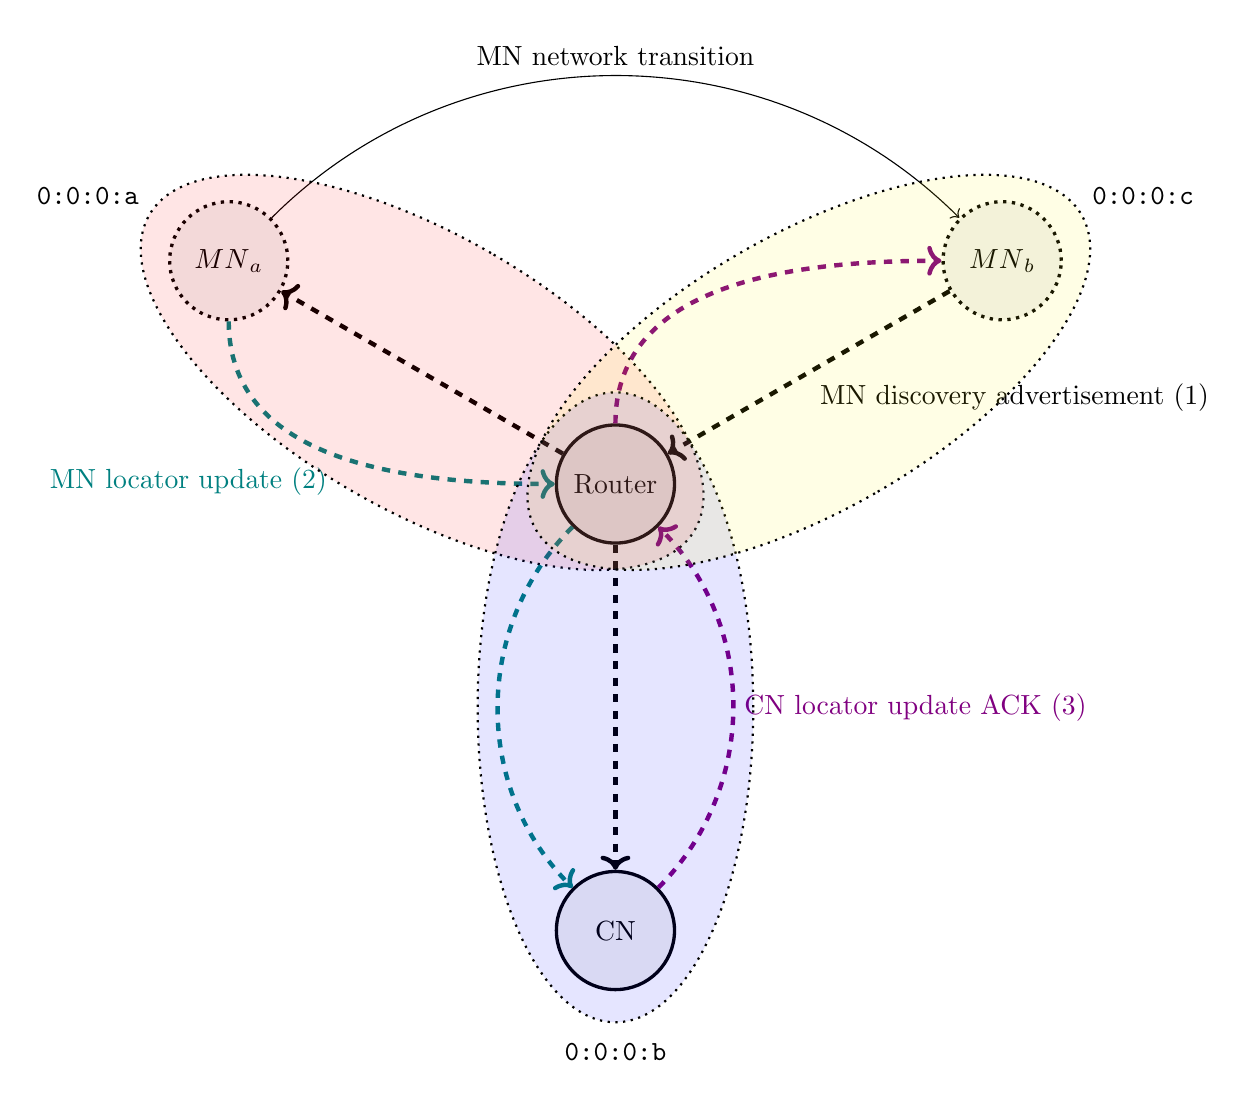
\begin{tikzpicture}[
    nwknode/.style={
        circle,
        very thick,
        minimum size=1.5cm,
        draw,
        fill=black!5,
    },
    network/.style args = {#1}{
        draw,
        ellipse,
        minimum height=8cm,
        minimum width=3.5cm,
        inner xsep=0mm, 
        inner ysep=3mm,
        thick,
        dotted,
        fill=#1,
        fill opacity=0.1,
        text opacity=1,
    }
]

\begin{scope}
    \node[regular polygon, regular polygon sides=3, inner sep=2cm, rotate=60] (a) {};
    \node[regular polygon, regular polygon sides=3, inner sep=2cm] (c) {};
    
    \node[nwknode] (r) at (a) {Router};
    \node[nwknode] (cn)  at (a.corner 2) {CN};
    \node[nwknode, dotted] (mn_a)  at (a.corner 1) {$\text{MN}_a$};
    \node[nwknode, dotted] (mn_b)  at (a.corner 3) {$\text{MN}_b$};
    
    \draw[->] (mn_a) to[out=45,in=135] node[above] {MN network transition} (mn_b);
    
    \draw[ultra thick,dashed,->] (mn_b) -- node[below right] {MN discovery advertisement (1)} (r);
    \draw[ultra thick,dashed,->] (r) -- node[right] {} (cn);
    \draw[ultra thick,dashed,->] (r) -- node[right] {} (mn_a);
    
    \draw[ultra thick,dashed,teal,->] (mn_a) to[out=-90,in=180] node[below left] {MN locator update (2)} (r);
    \draw[ultra thick,dashed,teal,->] (r) to[out=-135,in=135] node[left] {} (cn);
    
    \draw[ultra thick,dashed,violet,->] (cn) to[out=45,in=-45] node[right] {CN locator update ACK (3)} (r);
    \draw[ultra thick,dashed,violet,->] (r) to[out=90,in=180] node[below right] {} (mn_b);
    
    % horribly hacky
    \node[network={red}, rotate=60, label=\texttt{0:0:0:a}] at (c.side 1) {};
    \node[network={blue}, rotate=0, label={[anchor=south,above=-6mm]270:\texttt{0:0:0:b}}] at (c.side 2) {};
    \node[network={yellow}, rotate=-60, label=\texttt{0:0:0:c}] at (c.side 3) {};
\end{scope}

\end{tikzpicture}
}} &
            \subfloat[Sequence Diagram \label{fig:locator_update_sequence_diagram}]
                {\scalebox{0.4}{
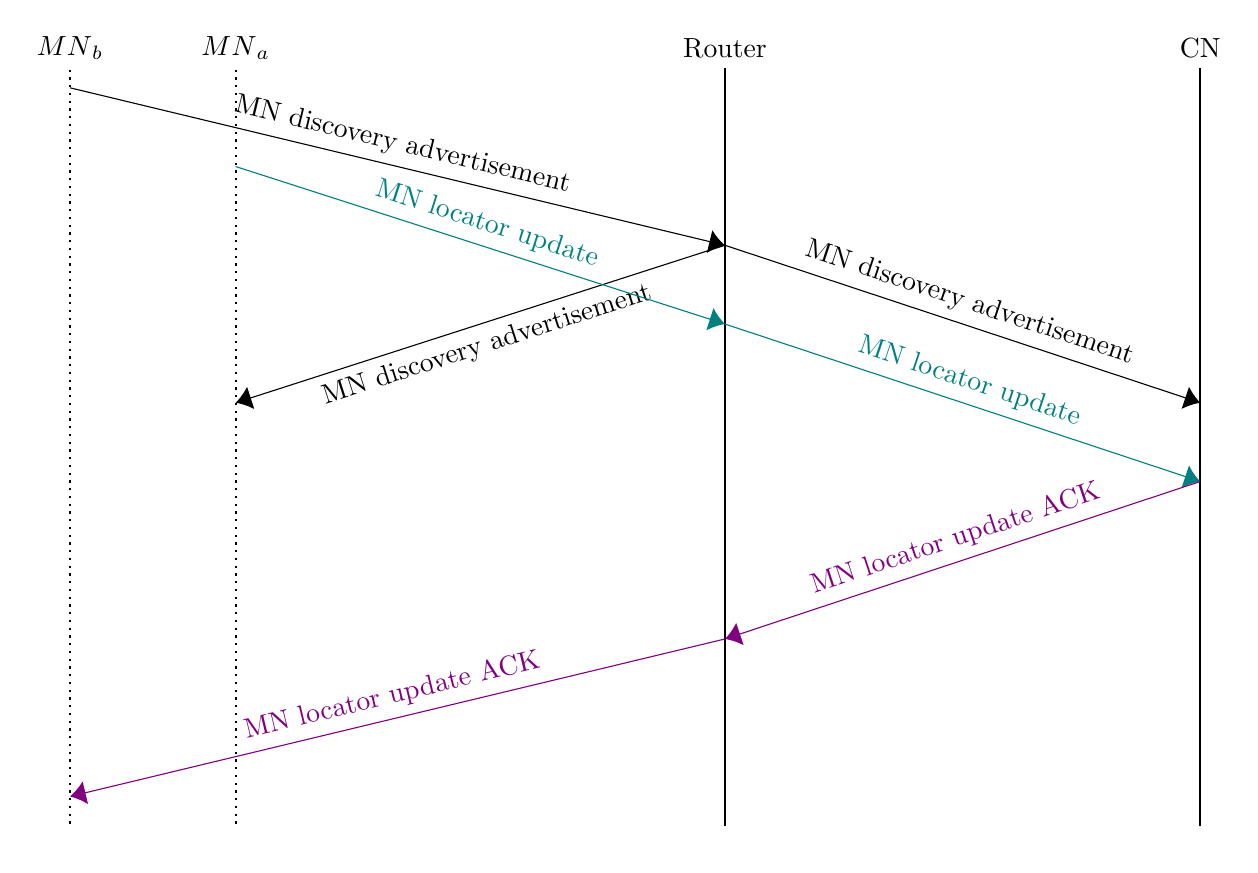
\begin{tikzpicture}[]
    \node[] (r) {Router};
    \node[right = 5cm of r] (cn) {CN};
    \node[left = 5cm of r] (mna) {$\text{MN}_a$};
    \node[left = 1cm of mna] (mnb) {$\text{MN}_b$};
    \node[below of=r, node distance=10cm] (r_ground) {};
    \node[below of=cn, node distance=10cm] (cn_ground) {};
    \node[below of=mnb, node distance=10cm] (mnb_ground) {};
    \node[below of=mna, node distance=10cm] (mna_ground) {};
    %
    \draw[thick] (r) -- (r_ground);
    \draw[thick] (cn) -- (cn_ground);
    \draw[dotted, thick] (mnb) -- (mnb_ground);
    \draw[dotted, thick] (mna) -- (mna_ground);
    
    
    
    
    \draw[-{Latex[length=2mm,width=3mm]}] ($(mnb)!0.05!(mnb_ground)$) -- node[above,sloped]{MN discovery advertisement}  ($(r)!0.25!(r_ground)$);
    \draw[-{Latex[length=2mm,width=3mm]}] ($(r)!0.25!(r_ground)$) -- node[below,sloped]{MN discovery advertisement}  ($(mna)!0.45!(mna_ground)$);
    \draw[-{Latex[length=2mm,width=3mm]}] ($(r)!0.25!(r_ground)$) -- node[above,sloped]{MN discovery advertisement}  ($(cn)!0.45!(cn_ground)$);
    
    \draw[-{Latex[length=2mm,width=3mm]},teal] ($(mna)!0.15!(mna_ground)$) -- node[above,sloped]{MN locator update}  ($(r)!0.35!(r_ground)$);
    \draw[-{Latex[length=2mm,width=3mm]},teal] ($(r)!0.35!(r_ground)$) -- node[above,sloped]{MN locator update}  ($(cn)!0.55!(cn_ground)$);
    
    \draw[-{Latex[length=2mm,width=3mm]},violet] ($(cn)!0.55!(cn_ground)$) -- node[above,sloped]{MN locator update ACK}  ($(r)!0.75!(r_ground)$);
    \draw[-{Latex[length=2mm,width=3mm]},violet] ($(r)!0.75!(r_ground)$) -- node[above,sloped]{MN locator update ACK}  ($(mnb)!0.95!(mnb_ground)$);
    
\end{tikzpicture}
}} \\
        \end{tabular}
    }
    \caption{Locator Update Example}
    \label{fig:locator_udpate}
\end{figure}
\end{frame}

\begin{frame}{Physical Testbed}
\begin{figure}[ht]
    \centering
    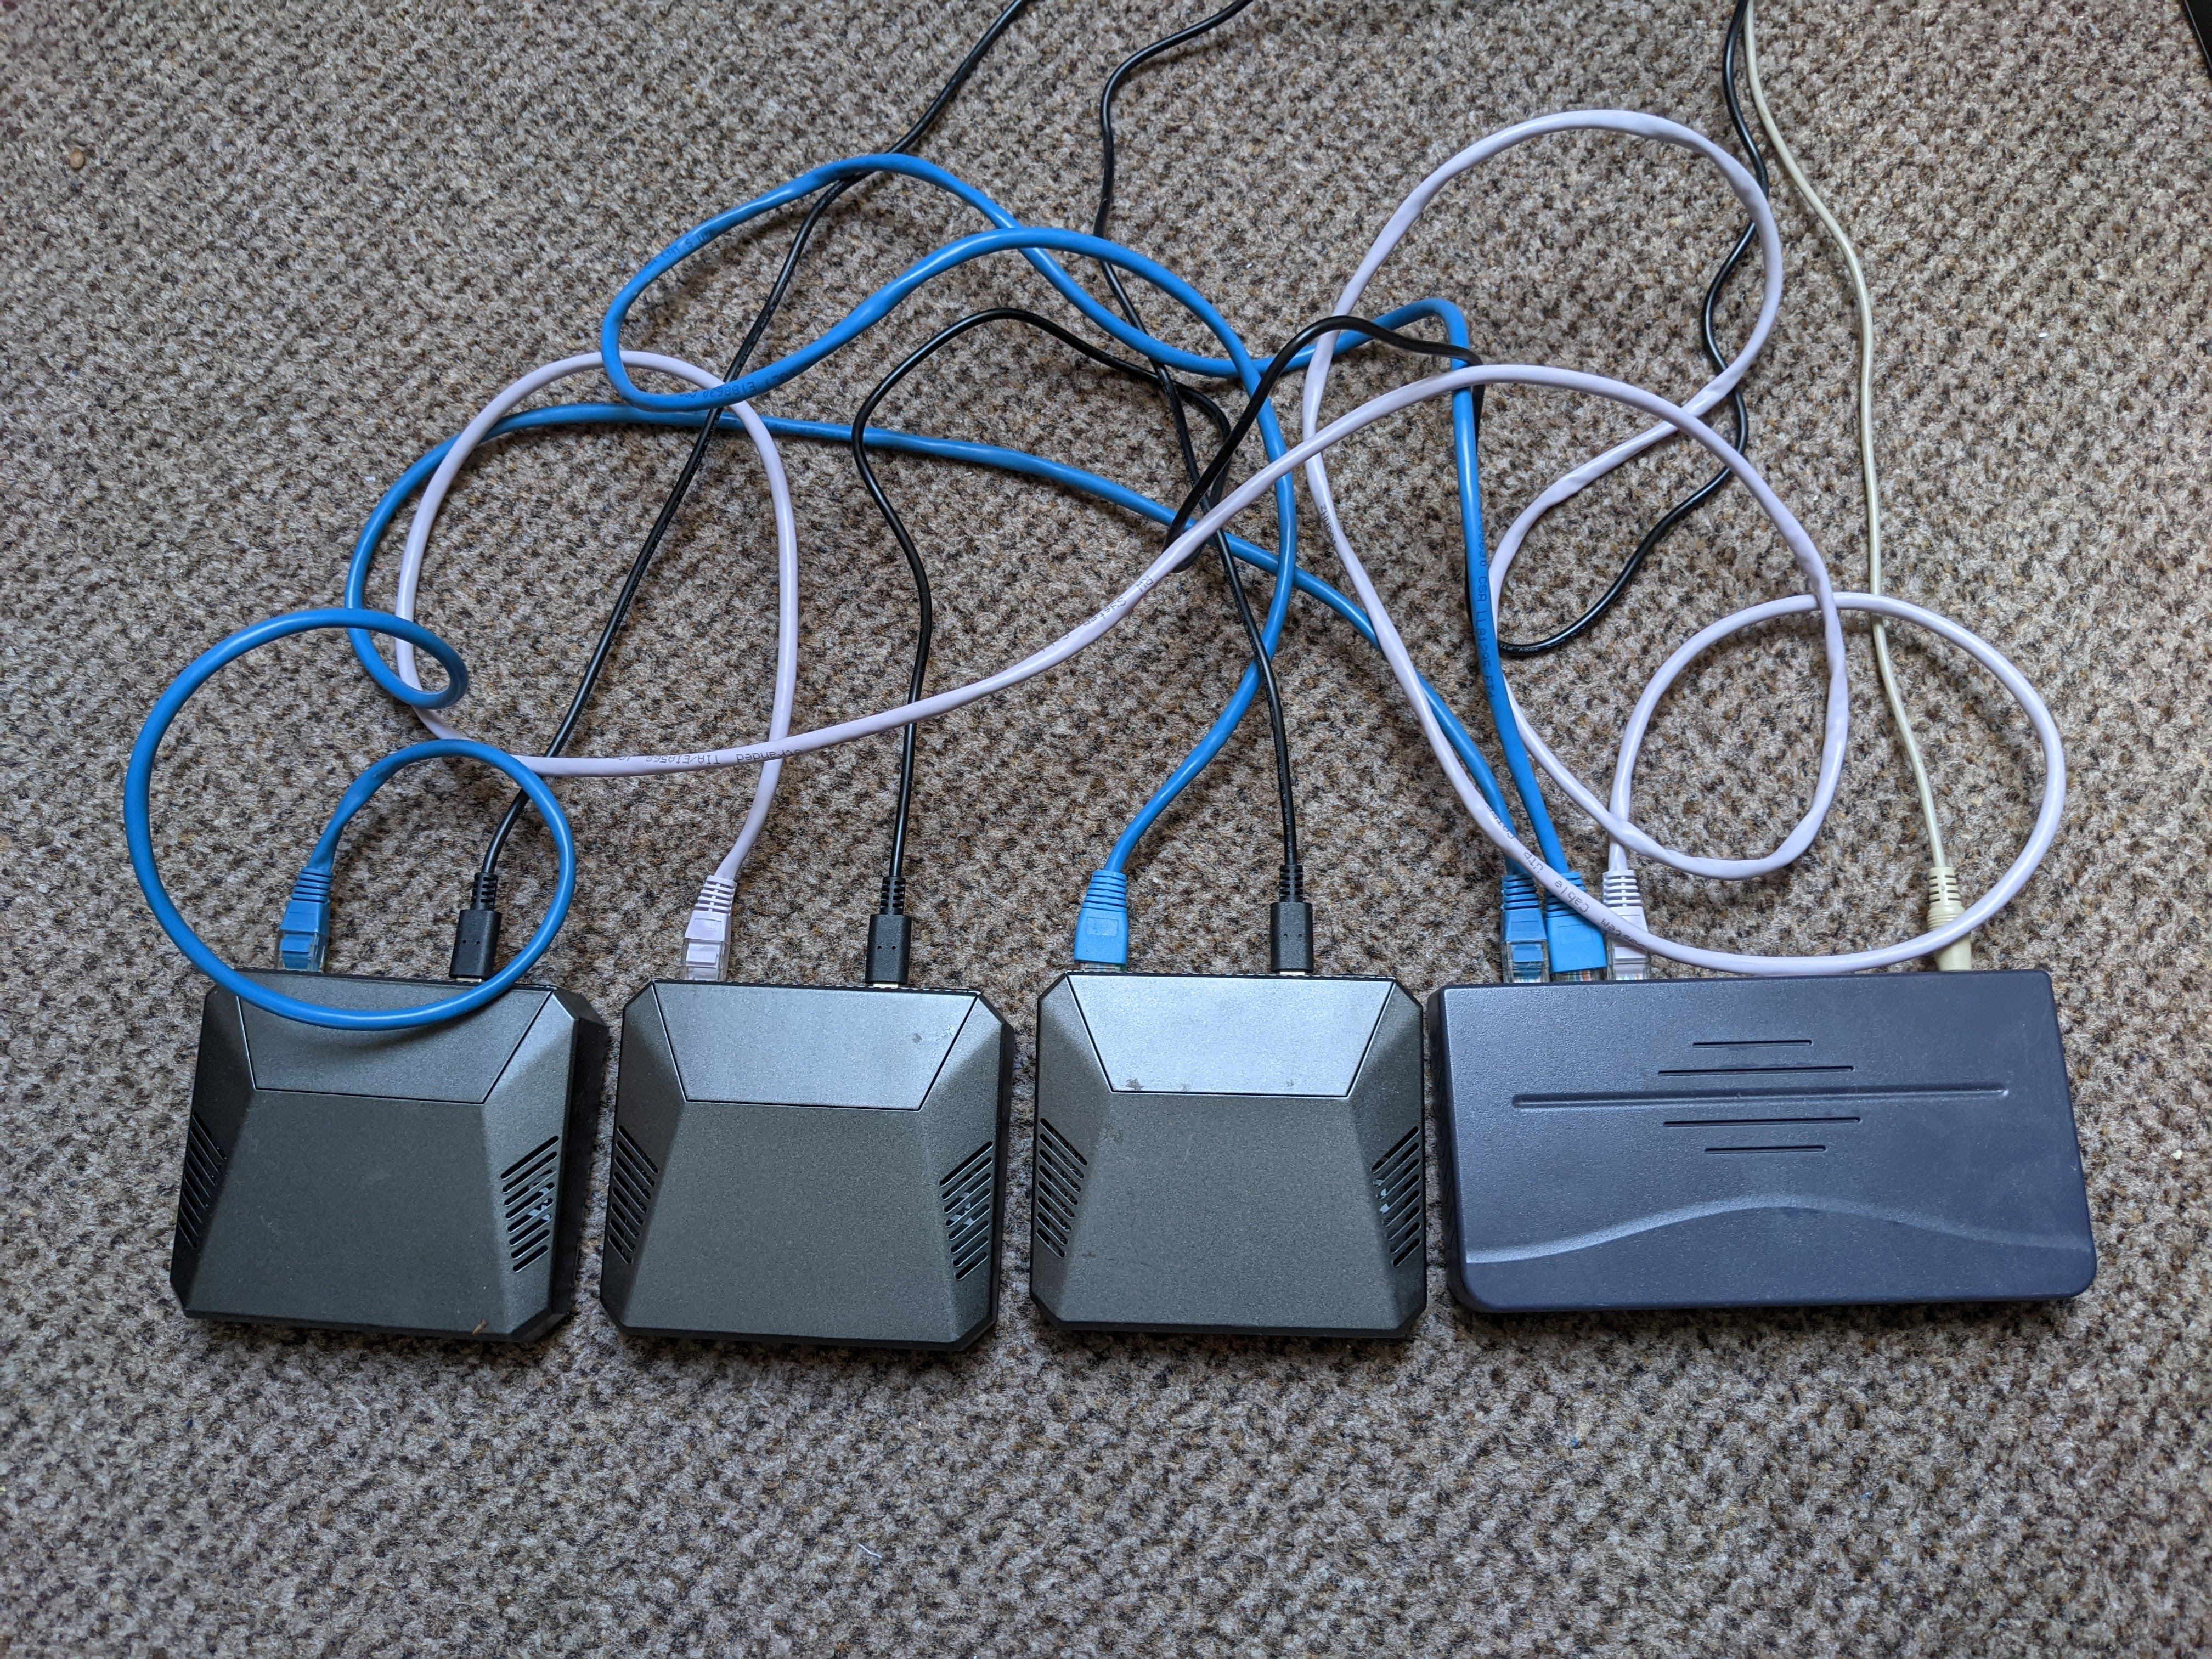
\includegraphics[width = 0.75\textwidth]{testbed.jpg}
    \caption{Physical Testbed}
    \label{fig:physical_testbed}
\end{figure}
\end{frame}

\begin{frame}{Experiment Virtual Topology}
\begin{figure}[ht]
    \centering
    \scalebox{0.35}{
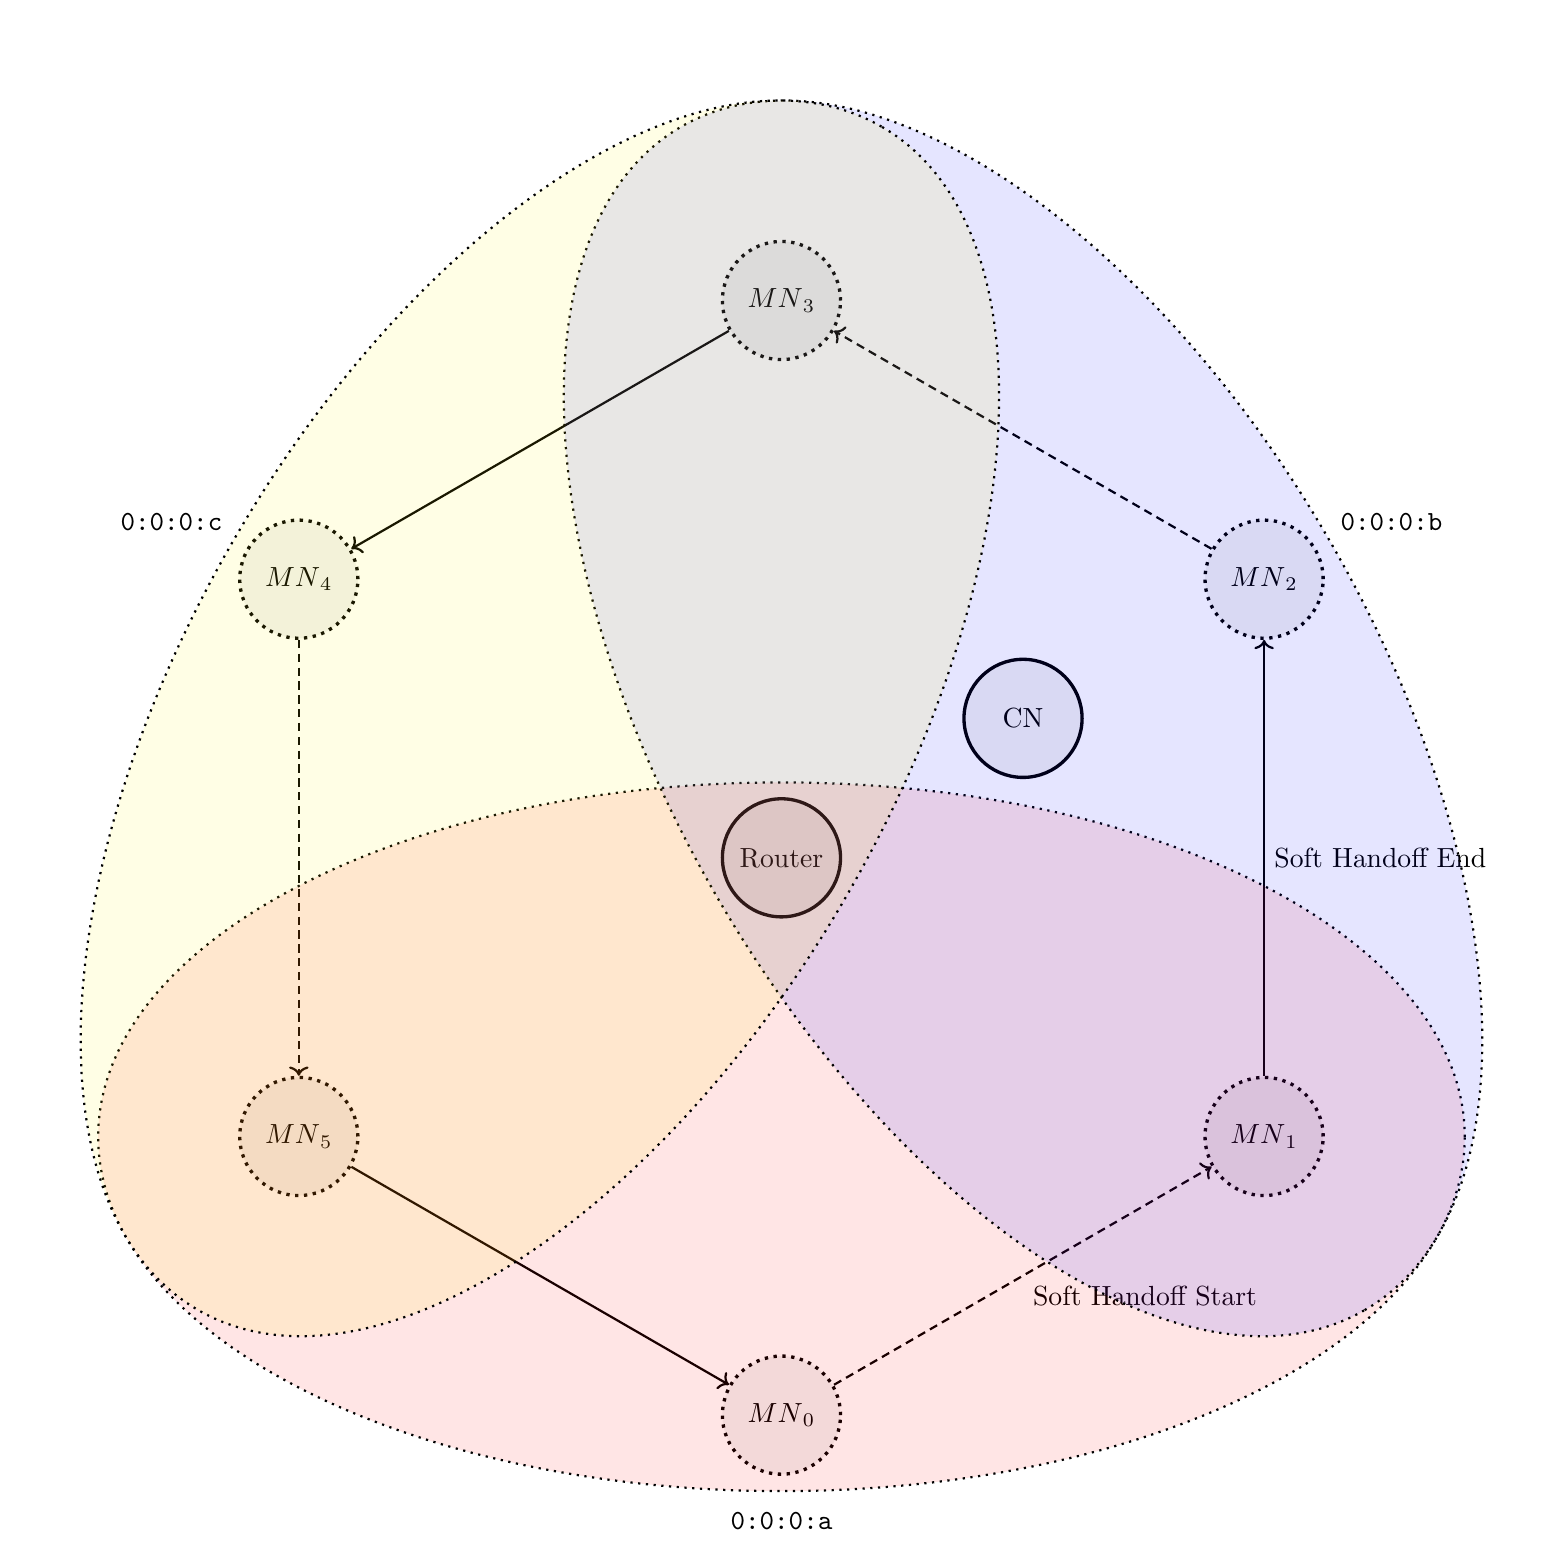
\begin{tikzpicture}[
    nwknode/.style={
        circle,
        very thick,
        minimum size=1.5cm,
        draw,
        fill=black!5,
    },
    network/.style args = {#1}{
        fit=(a.corner 2) (a.corner 3), 
        draw,
        ellipse,
        minimum height=9cm,
        inner xsep=0mm, 
        inner ysep=3mm,
        thick,
        dotted,
        fill=#1,
        fill opacity=0.1,
        text opacity=1,
        % 
    }
]
    \node[regular polygon, regular polygon sides=3, inner sep=2.5cm] (a) {};
    \node[regular polygon, regular polygon sides=6, inner sep=5cm]   (b) {};
    
    \node[nwknode, dotted] (mn0) at (b.side 4) {$\text{MN}_0$};
    \node[nwknode, dotted] (mn1) at (b.side 5) {$\text{MN}_1$};
    \node[nwknode, dotted] (mn2) at (b.side 6) {$\text{MN}_2$};
    \node[nwknode, dotted] (mn3) at (b.side 1) {$\text{MN}_3$};
    \node[nwknode, dotted] (mn4) at (b.side 2) {$\text{MN}_4$};
    \node[nwknode, dotted] (mn5) at (b.side 3) {$\text{MN}_5$};
    \node[nwknode] (cn)  at (a.side 3) {CN};
    
    \draw[->, thick, densely dashed] (mn0) -- node[below right] {Soft Handoff Start} (mn1);
    \draw[->, thick] (mn1) -- node[right] {Soft Handoff End} (mn2);
    \draw[->, thick, densely dashed] (mn2) -- (mn3);
    \draw[->, thick] (mn3) -- (mn4);
    \draw[->, thick, densely dashed] (mn4) -- (mn5);
    \draw[->, thick] (mn5) -- (mn0);
    
    \node[nwknode] (router) at (a) {Router};
    
    \node[network={red}, label={[anchor=south,above=-6mm]270:\texttt{0:0:0:a}}] {};
    \node[network={blue}, rotate=-60, label=\texttt{0:0:0:b}] at (a.side 3) {};
    \node[network={yellow}, rotate=60, label=\texttt{0:0:0:c}] at (a.side 1) {};

\end{tikzpicture}
}
    \caption{Experiment Virtual Topology}
    \label{fig:experiment_topology}
\end{figure}
\end{frame}






\end{document}
